\section{Resultados}\label{sec:resultados}

\subsection{Referencia histórica ya consultada}
Los 2\,232 registros de 2024--2025 contienen 222 multifatales. Este periodo no es un test nuevo: ya fue consultado y no autoriza reajustes. La finalidad del bundle no crea independencia científica. El cuadro~\ref{tab:metricas-referencia} reúne el desempeño en ambas escalas de probabilidad.

\begin{table}[tbp]\centering\caption{Métricas del modelo canónico en la referencia histórica. Los intervalos son percentiles bootstrap al 95\,\% sobre remuestreo de filas con predicciones congeladas.}\label{tab:metricas-referencia}\begin{tabular}{lcc}\toprule
Métrica & Cruda, $t=0.65$ & Platt, $t=0.15$ \\\midrule
PR-AUC & 0.3254 [0.2703, 0.3871] & 0.3254 [0.2703, 0.3871] \\
ROC-AUC & 0.7916 [0.7595, 0.8227] & 0.7916 [0.7595, 0.8227] \\
F1 & 0.4030 [0.3496, 0.4487] & 0.3989 [0.3523, 0.4423] \\
Precisión & 0.3025 & 0.2830 \\
Recall & 0.6036 & 0.6757 \\
Brier & 0.1642 & 0.0777 \\
ECE & 0.2338 & 0.0133 \\\midrule
\emph{Accuracy} (solo referencia) & 0.8221 & 0.7975 \\\bottomrule
\end{tabular}\end{table}

La \emph{accuracy} se reporta por coherencia con el protocolo predeclarado, y su lectura confirma exactamente por qué se descartó como criterio de calidad: un clasificador que respondiera siempre ``letalidad simple'' alcanzaría 0.9005 en esta misma partición, es decir, más que cualquiera de las dos escalas del modelo, sin identificar un solo siniestro multifatal. La escala calibrada exhibe menor \emph{accuracy} que la cruda precisamente porque acepta más falsas alertas a cambio de recuperar más positivos.

Platt mejora la escala, no el ranking. La matriz calibrada contiene 1\,630 TN, 380 FP, 72 FN y 150 TP. El mayor recall se obtiene a costa de más falsas alertas; no se presenta como desempeño excelente.

\subsection{Capacidad de ordenamiento}
Las curvas de la figura~\ref{fig:curvas-pr-roc} separan la capacidad de ordenamiento del punto de decisión. La curva precisión-recall se lee contra la prevalencia de 0.099: la precisión se mantiene entre 0.30 y 0.40 en el rango de recall 0.2--0.7, es decir, tres a cuatro veces la línea base, pero nunca alcanza valores altos. La curva ROC muestra el comportamiento típico de una señal moderada, con la mayor ganancia concentrada en el primer 20\,\% de falsos positivos.

\begin{figure}[tbp]
\centering
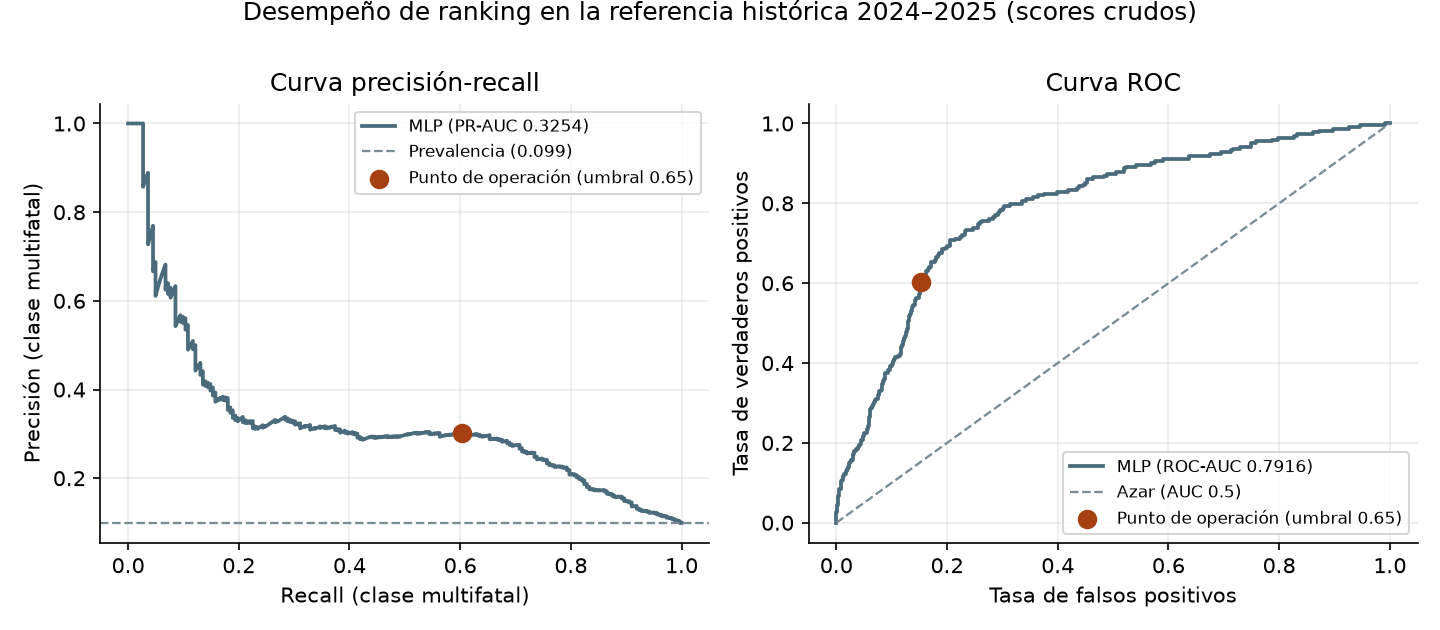
\includegraphics[width=\textwidth]{figures/fig17_pr_roc_curves.png}
\caption{Curvas precisión-recall y ROC sobre los scores crudos de la referencia histórica. El punto de operación corresponde al umbral 0.65 fijado en 2023: recall 0.604 con precisión 0.302, sobre una tasa de falsos positivos de 0.154.}
\label{fig:curvas-pr-roc}
\end{figure}

\subsection{Calibración y estructura del error}
La figura~\ref{fig:confiabilidad} contrasta ambas escalas de probabilidad. La sigmoide cruda es sistemáticamente optimista: en todos los bins la frecuencia observada queda por debajo de la diagonal, con ECE 0.2338. Tras Platt, los bins con soporte suficiente se alinean con la diagonal y el ECE baja a 0.0133. Los bins superiores de la escala calibrada reúnen entre 1 y 9 registros, por lo que su desviación aparente no es evidencia de descalibración.

La figura~\ref{fig:matrices-confusion} traduce esa diferencia de escala en conteos de decisión y hace visible el intercambio que impone el umbral.

\begin{figure}[tbp]
\centering
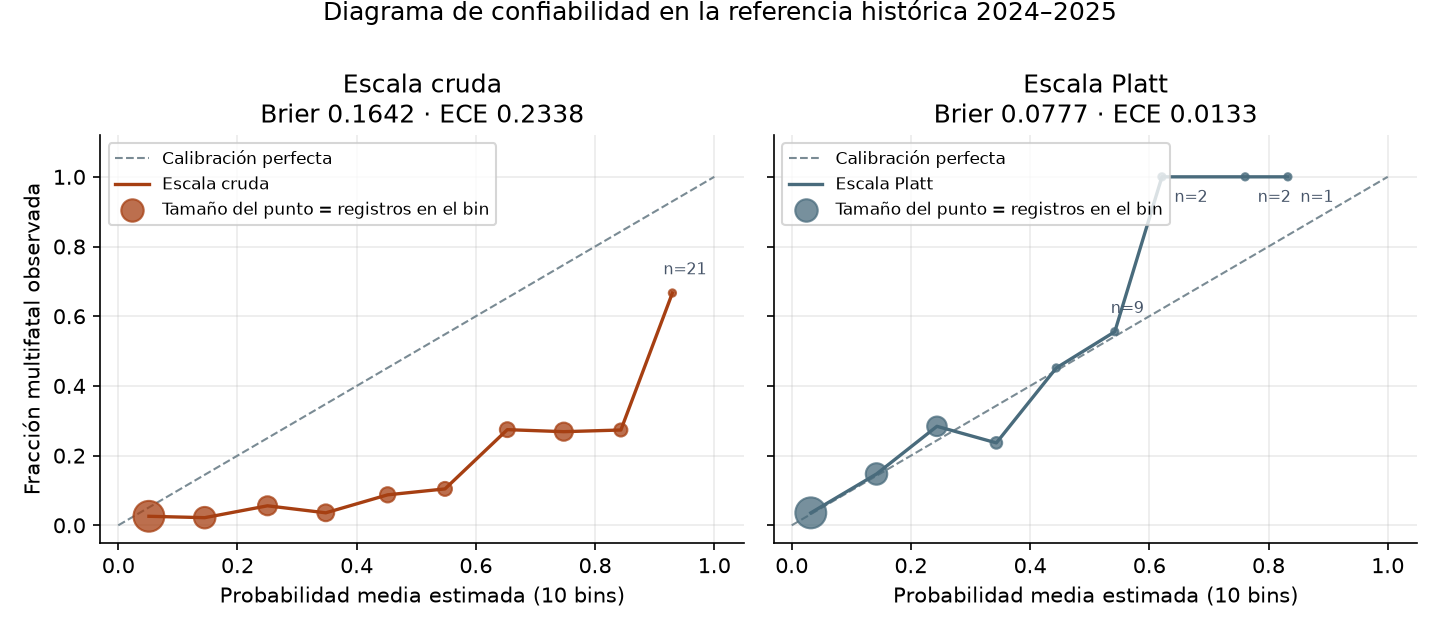
\includegraphics[width=\textwidth]{figures/fig15_reliability_diagram.png}
\caption{Diagrama de confiabilidad por decil de probabilidad. El tamaño del punto es proporcional al número de registros del bin; se anota $n$ cuando el bin reúne 25 registros o menos.}
\label{fig:confiabilidad}
\end{figure}

\begin{figure}[tbp]
\centering
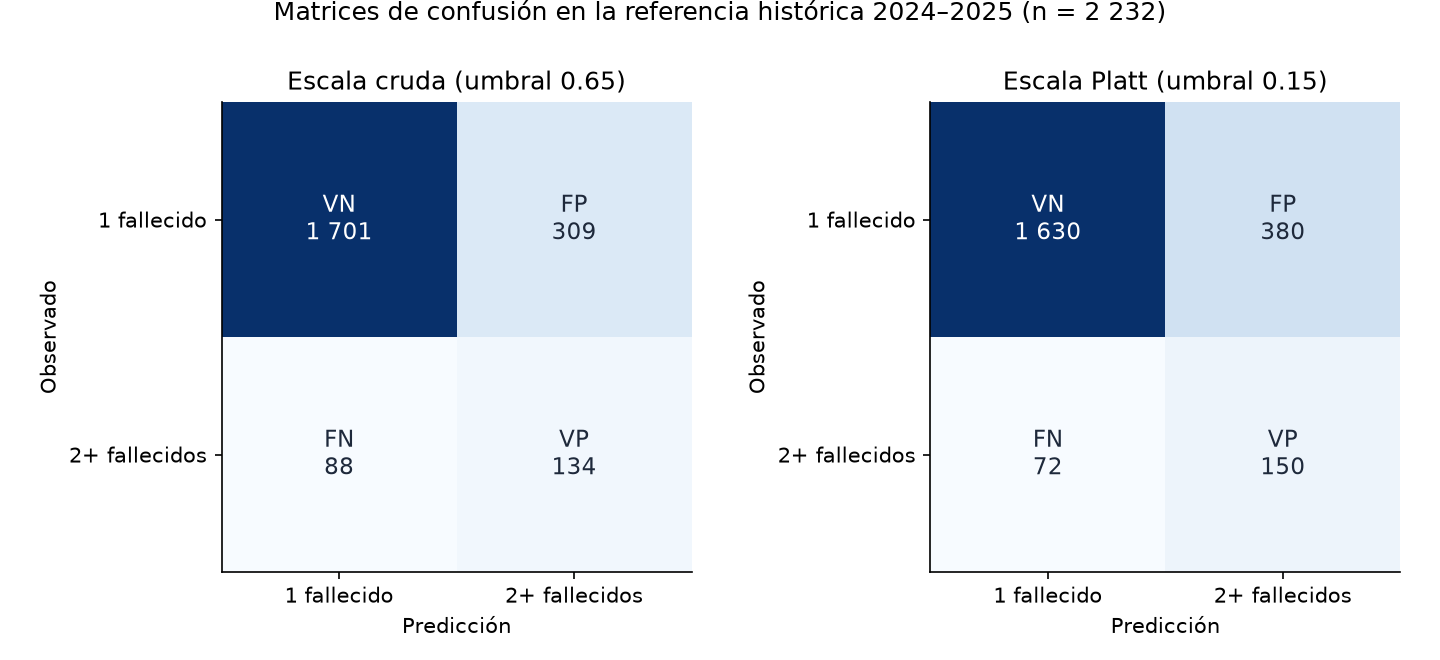
\includegraphics[width=\textwidth]{figures/fig16_confusion_matrices.png}
\caption{Matrices de confusión en ambas escalas. El umbral calibrado convierte 16 falsos negativos en verdaderos positivos (de 88 a 72) al precio de 71 falsas alertas adicionales (de 309 a 380): el desplazamiento de umbral redistribuye el error, no lo elimina.}
\label{fig:matrices-confusion}
\end{figure}

\begin{figure}[tbp]
\centering
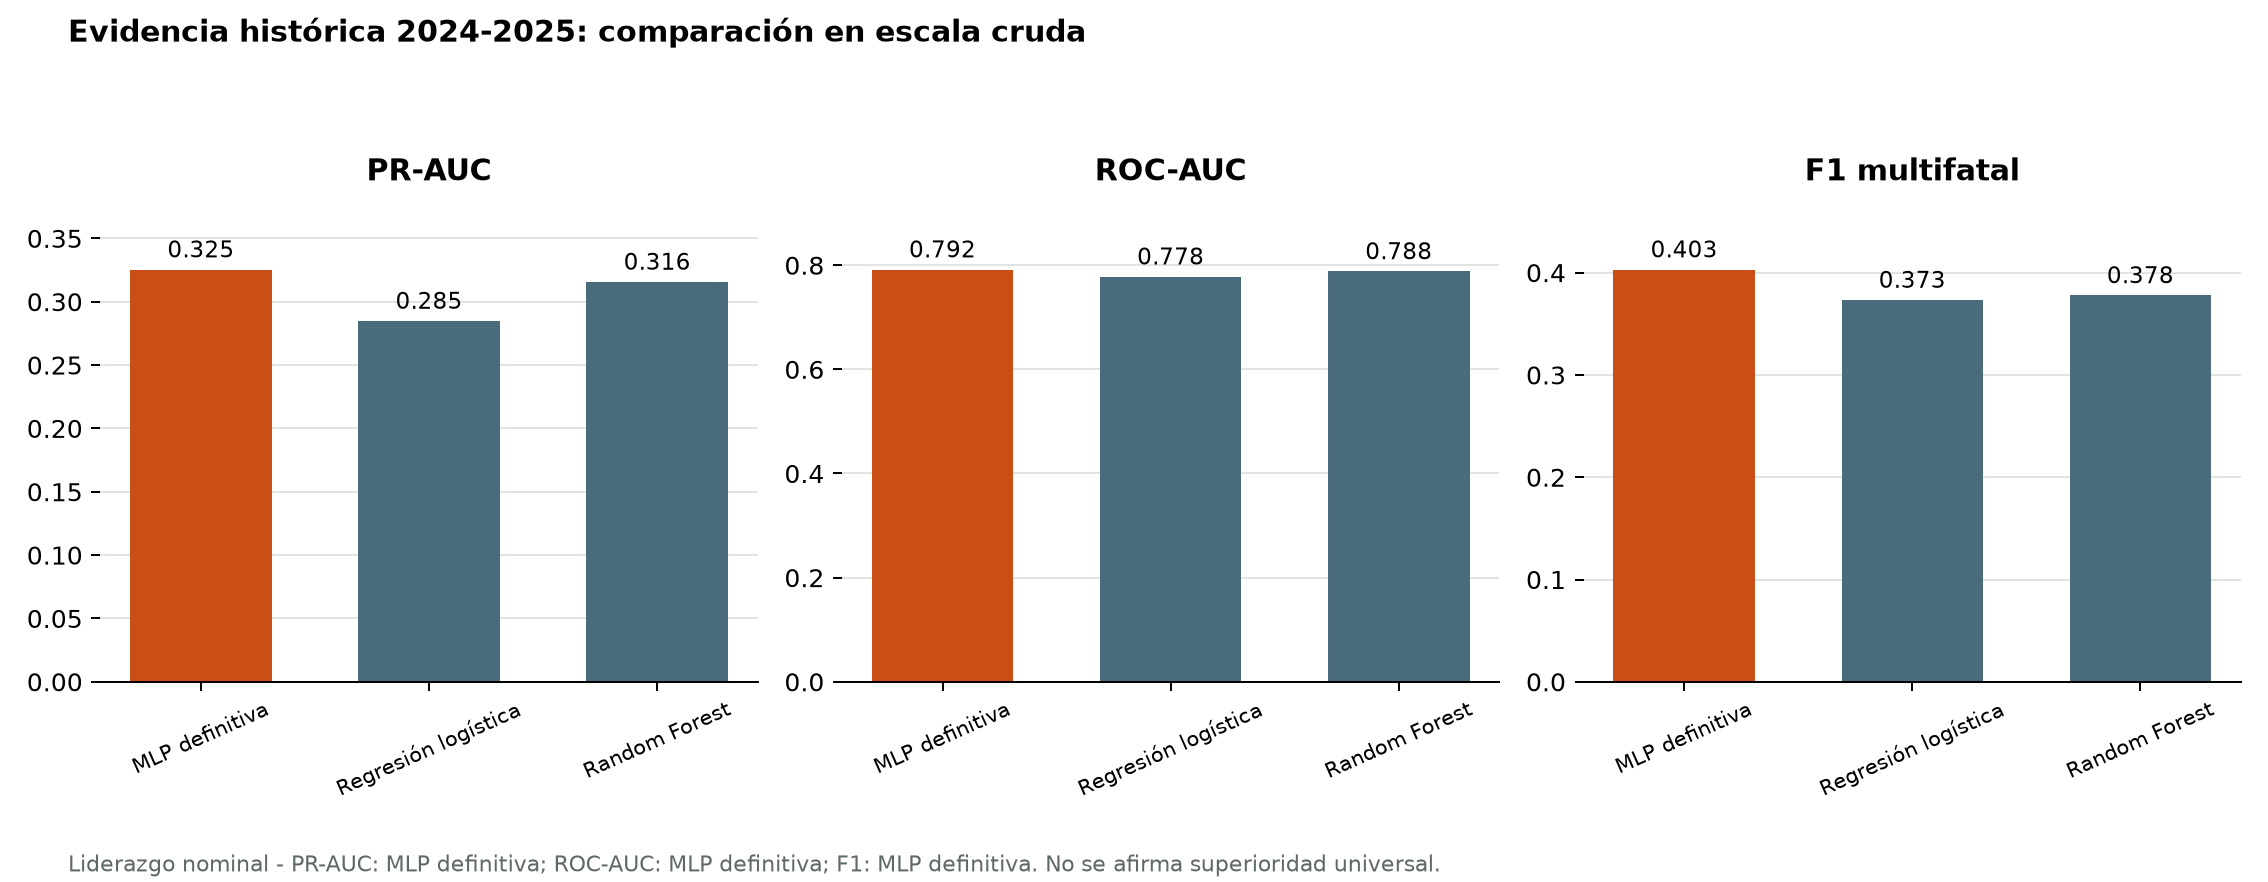
\includegraphics[width=\textwidth]{figures/final_model_evidence.png}
\caption{Comparación descriptiva en la referencia histórica 2024--2025 sobre scores crudos. El liderazgo nominal no equivale a superioridad universal.}
\label{fig:evidencia-referencia}
\end{figure}

\subsection{Separabilidad y elección del umbral}
Las métricas agregadas no muestran cuánto se solapan las dos clases ni por qué el umbral se sitúa donde se sitúa. La figura~\ref{fig:separabilidad} responde ambas cosas. El panel izquierdo superpone la distribución de la probabilidad calibrada según la clase observada, en escala logarítmica para que la clase minoritaria sea visible: las dos distribuciones se solapan de forma sustancial por debajo de 0.2, pero por encima de 0.35 los siniestros multifatales dominan, y prácticamente todos los casos con probabilidad superior a 0.55 pertenecen a esa clase. Ese es el origen de una PR-AUC moderada acompañada de un ordenamiento útil.

El panel derecho recorre la grilla completa de umbrales. La precisión crece de forma monótona y el \emph{recall} decrece, como corresponde, y el F1 describe una meseta amplia entre 0.12 y 0.22 en lugar de un pico estrecho. El umbral 0.15, fijado en 2023 sin observar este periodo, cae dentro de esa meseta; el máximo de F1 sobre la referencia se alcanza en 0.17. Que la diferencia entre el umbral elegido a ciegas y el óptimo observado a posteriori sea de dos centésimas es evidencia de que la política de decisión se transfiere entre periodos.

\begin{figure}[tbp]
\centering
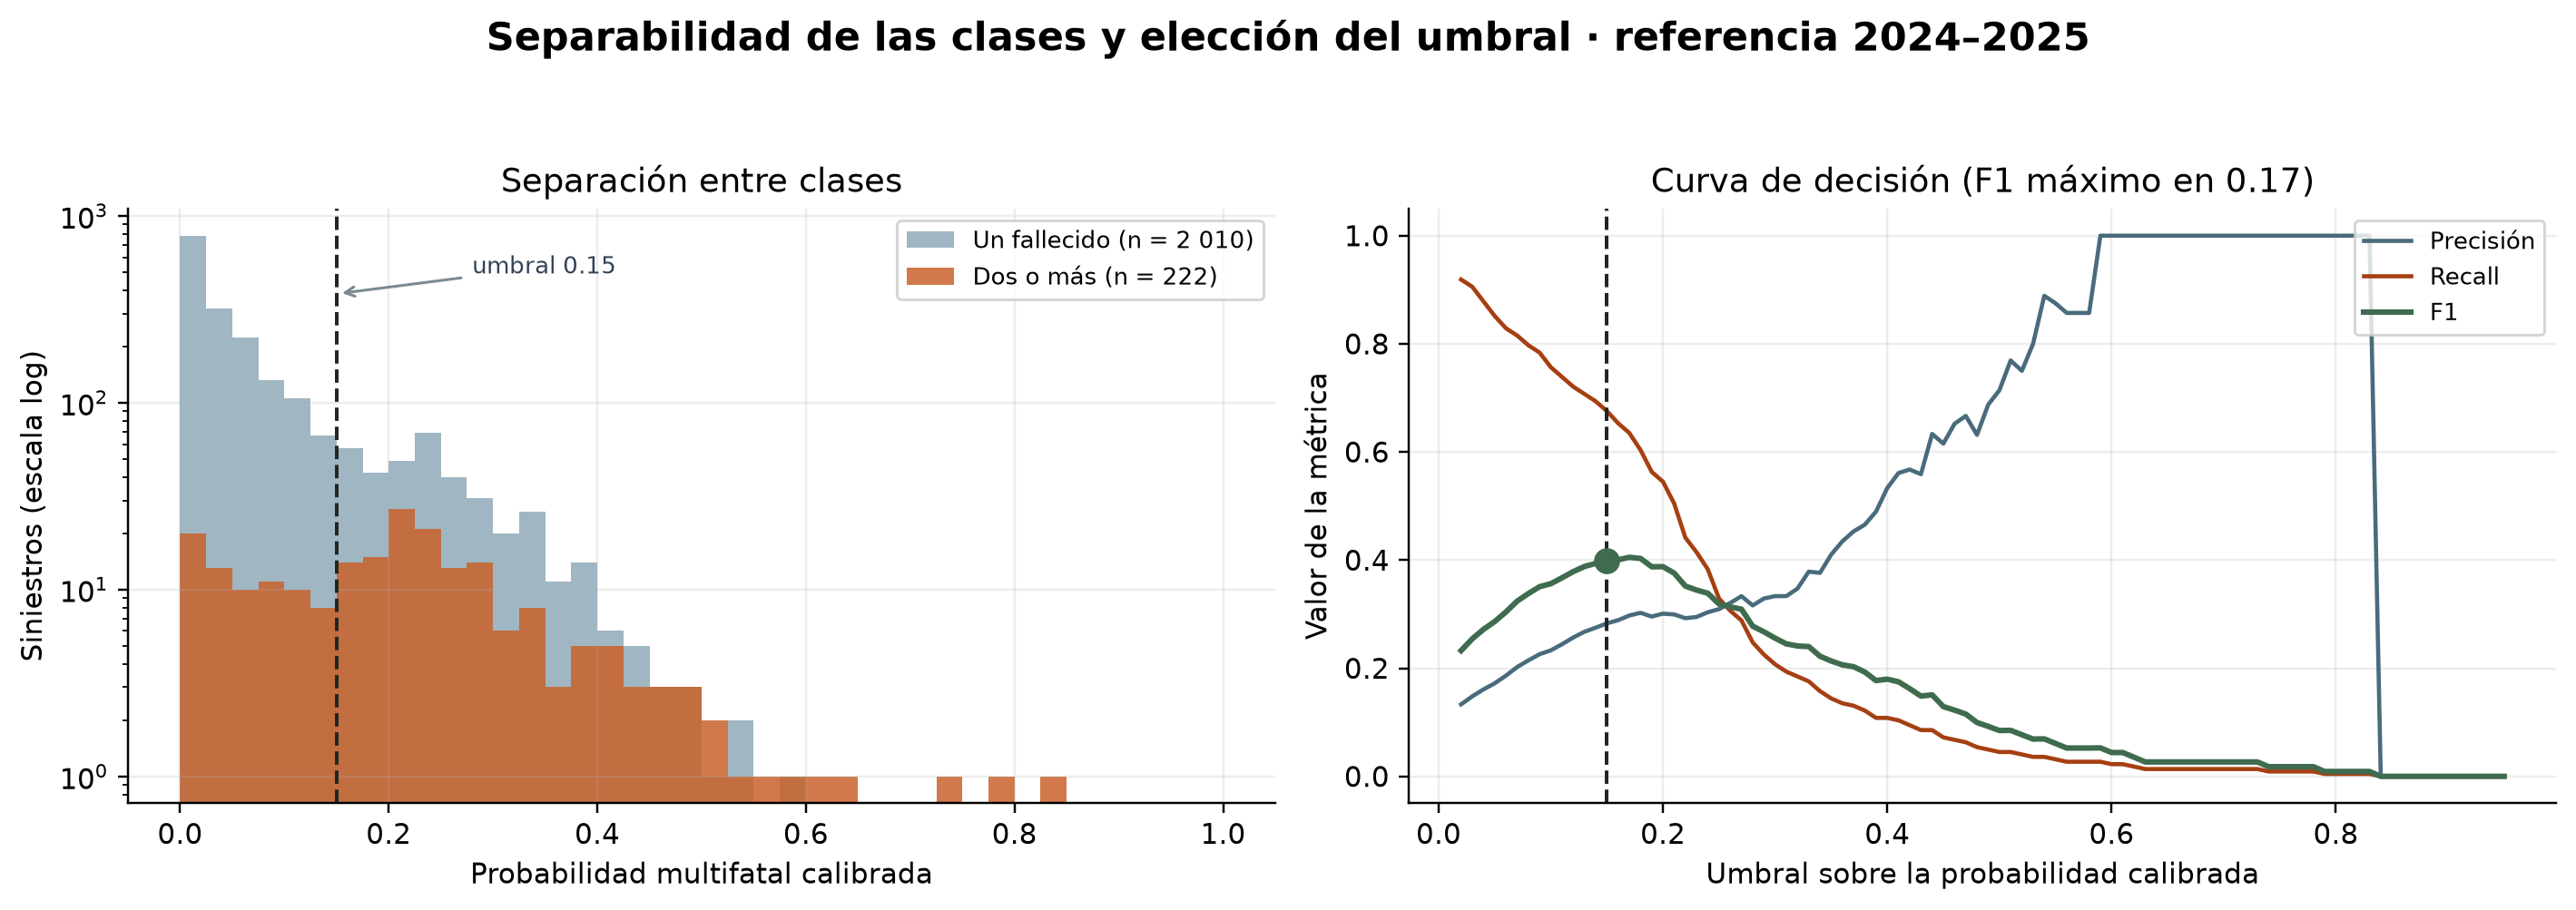
\includegraphics[width=\textwidth]{figures/fig18_separability_threshold.png}
\caption{Separabilidad de las clases y curva de decisión. El punto verde marca el umbral canónico de 0.15 sobre la curva de F1; la meseta a su alrededor indica que la decisión no es frágil ante pequeños desplazamientos del umbral.}
\label{fig:separabilidad}
\end{figure}

\subsection{Valor del ordenamiento y estabilidad por segmento}
Para un uso realista importa menos la clase declarada que la capacidad de ordenar. La curva de ganancia acumulada de la figura~\ref{fig:ganancia} expresa esa capacidad en términos operativos: revisando el 10\,\% de los siniestros con mayor probabilidad se recupera el 32\,\% de los multifatales; revisando el 20\,\%, el 61\,\%; y revisando el 30\,\%, el 74\,\%. Frente a un orden aleatorio, que recuperaría respectivamente el 10, el 20 y el 30\,\%, el modelo triplica el rendimiento en el primer tramo.

\begin{figure}[tbp]
\centering
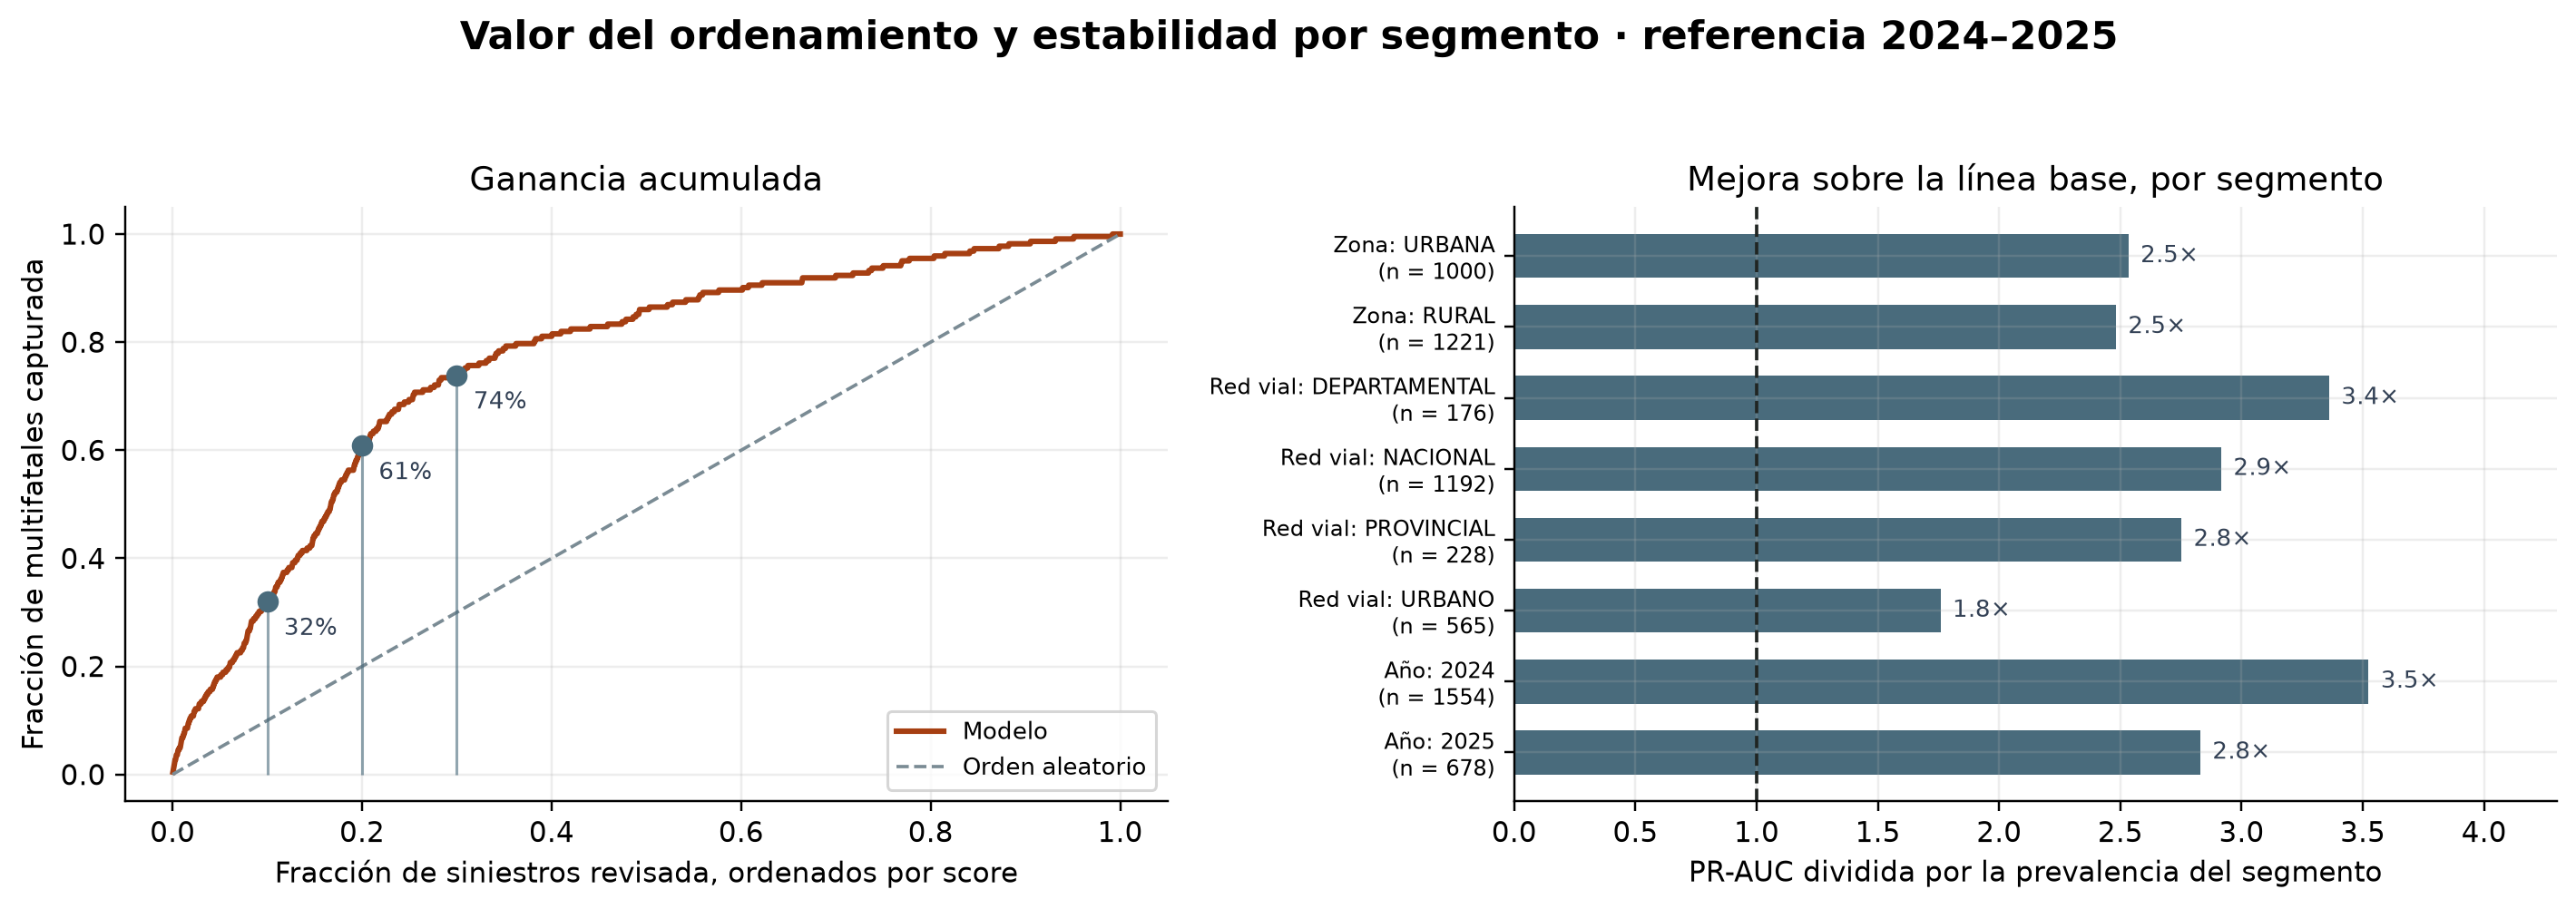
\includegraphics[width=\textwidth]{figures/fig19_gain_segments.png}
\caption{Ganancia acumulada y desempeño por segmento. La mejora se expresa como PR-AUC dividida por la prevalencia del propio segmento, de modo que segmentos con distinta proporción de multifatales resulten comparables; el valor 1 corresponde a no aportar información.}
\label{fig:ganancia}
\end{figure}

El panel derecho comprueba que esa capacidad no depende de un segmento particular. La mejora sobre la prevalencia se mantiene entre 1.8 y 3.5 veces en todas las particiones examinadas ---por zona, por red vial y por año---, de modo que ningún grupo queda por debajo de la línea base. El extremo inferior corresponde a la red vial urbana, con 1.8 veces sobre una prevalencia de 0.034: es el entorno donde el modelo aporta menos, coherentemente con que la multifatalidad urbana sea un fenómeno poco frecuente y menos ligado al contexto vial. El extremo superior es la red departamental, con 3.4 veces. La comparación entre 2024 y 2025 (3.5 y 2.8) sugiere además cierto deterioro en el periodo más reciente, que conviene vigilar en futuras versiones y que es coherente con su carácter preliminar.

\subsection{Baselines}
La figura~\ref{fig:evidencia-referencia} compara la MLP con las líneas base clásicas en las tres métricas principales sobre la escala cruda. Las tres barras de cada panel están próximas entre sí, lo que anticipa el resultado del análisis pareado: el liderazgo nominal de la red no equivale a superioridad estadística.

Las tres líneas base se implementaron con scikit-learn \cite{pedregosa_scikit_2011} sobre el mismo contrato de variables y la misma política de umbral. El DummyClassifier usa \texttt{strategy=prior}: probabilidad constante igual a la prevalencia de entrenamiento, no ``clase mayoritaria''. La MLP supera nominalmente a logística y Random Forest en esta referencia. El bootstrap pareado muestra ventaja nominal frente a logística en PR-AUC, ROC-AUC y F1; frente a Random Forest, PR-AUC y ROC-AUC incluyen cero. F1 es la excepción nominal: la diferencia MLP menos Random Forest es $+0.0252$, con IC 95\% $[0.00166,\,0.04790]$, favorable a la MLP. En total se inspeccionan seis comparaciones con IC 95\% nominales, sin ajuste por multiplicidad ni cobertura familiar simultánea. La inferencia es condicional a las predicciones y recetas congeladas; no establece superioridad universal ni incorpora incertidumbre de reentrenamiento.

\subsection{Diagnósticos rolling}
Los dos outer internos obtienen PR-AUC 0.3459/0.3259, ROC-AUC 0.7961/0.8090 y F1 0.3960/0.3677. La variación entre ventanas confirma que una sola partición no basta y refuerza la necesidad de validación externa.
